\section{Design Back-end}
In questa sezione sono illustrati i sistemi esterni con il quale la nostra applicazione dovrà interagire.
\begin{figure}[!h]
\centering
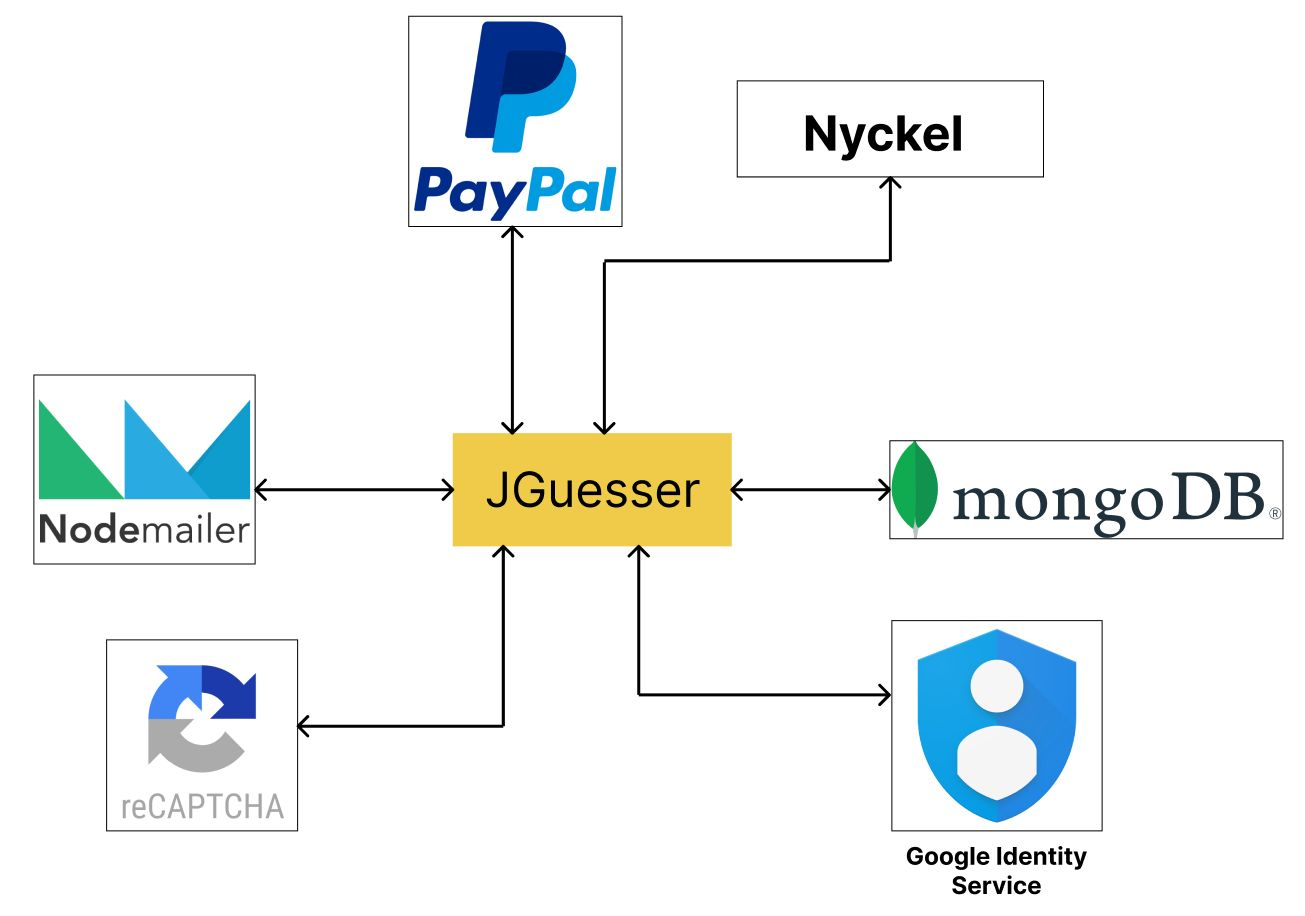
\includegraphics[scale=0.35]{images/back_end.jpg}
\caption{Schema del back-end}
\label{fig:schema_back-end}
\end{figure}

I sistemi esterni con la quale l'applicazione dovrà interfacciarsi sono i seguenti:
\begin{itemize}
    \item PayPal: sarà utilizzato come metodo di pagamento per acquistare la versione premium del servizio. L'applicazione JGuesser necessita quindi di interagire con il famoso servizio di pagamento, utilizzando le API che vengono fornite.
    \item Nyckel: machine learning API, che serviranno per classificare le immagine che l'utente disegnerà nel quiz Hiragana/Katakana di tipo 3. In questo modo il sistema sarà in grado di riconoscere se l'utente ha disegnato correttamente il simbolo relativo al suono oppure no.
    \item Nodemailer: API, che serviranno per inviare email all'utente, durante la fase di registrazione e di recupero della password, nel caso in cui egli l'abbia dimenticata.
    \item reCAPTCHA: questo servizio permette di distinguere essere umani da bot. Sarà quindi usato in fase di registrazione e recupero password, per proteggerci da spam e abusi. 
    \item Google Identity Service: questo servizio permetterà a tutti quelli utenti guest che vogliono utilizzare l'applicazione di registrarsi utilizzando un proprio account google.
    \item MongoDB: database che verrà utilizzato per memorizzare tutti i dati.
\end{itemize}